%!TEX program = xelatex
%%%%%%%%%%%%%%%%%%%%%%%这是导言部分的开始%%%%%%%%

%========= 导言部分声明文档的类型=================
\documentclass{article}

%=========导言部分可可以加载宏包=================
\usepackage{amsmath}                % 数学公式排版宏包
\usepackage{amssymb}                % 数学符号命令宏包
\usepackage{amsthm}                 % 数学定理宏包
\usepackage[UTF8]{ctex}             % 中文输入宏包
\usepackage[a4paper]{geometry}      % 页面设置宏包
\usepackage{setspace}               % 行间距宏包
\usepackage{graphicx}               % 图片宏包
\usepackage{listings}               % 代码宏包
\usepackage{color}					% 颜色宏包
\usepackage{xcolor}                 % 颜色处理宏包
\usepackage{float}                  % 浮动对象式样宏包
\usepackage{fontspec}
\usepackage{enumerate}				% 列举编号包

%=========页面设置==============================
\geometry{left=1cm,right=1cm,top=1cm,bottom=2cm}
\onehalfspacing
\setlength\parindent{0em}

%=========代码格式设置============================
\definecolor{dkgreen}{rgb}{0,0.6,0}
\definecolor{gray}{rgb}{0.5,0.5,0.5}
\definecolor{mauve}{rgb}{0.58,0,0.82}
% \setmonofont{Consolas}
\lstset{
	numbers = left, 	
	numberstyle = \color{gray}, 
	keywordstyle = \color{blue},
	commentstyle = \color{dkgreen}, 
	stringstyle = \color{mauve},
	basicstyle = \ttfamily,
	breaklines = true,
	frame = shadowbox, % 阴影效果
	rulesepcolor = \color{ red!20!green!20!blue!20} ,
	escapeinside = ``, % 英文分号中可写入中文
	xleftmargin = 2em,xrightmargin=2em, aboveskip=1em,
	framexleftmargin = 2em
} 

%=========导言部分可以定义标题信息===============
\title{组会报告}
\author{徐益}
\date{\today}
%%%%%%%%%%%%%%%%%%%%%%%这是导言部分的结束%%%%%%%%%

%%%%%%%%%%%%%%%%%%%%%%%这是正文部分的开始%%%%%%%%%
\begin{document}

%=========生成标题================================
\maketitle

%=========开始正文的输入==========================

%===========第一节=================
\section{工作内容}
1. 数据采集测试;

2. 低时延AVX2-LDPC译码实现;

% 3. 学习LDPC低时延译码方案。

%===========第一节=================
\section{数据采集测试}
\subsection{ramdisk}
\subsubsection{传统ramdisk}
% \lstset{language=C++}
\begin{lstlisting}
# mkdir /mnt/test
# mke2fs /dev/ram0
# mount /dev/ram /mnt/test
\end{lstlisting}
写入速率:700MB/s~800MB/s
\subsubsection{ramfs}
\begin{lstlisting}
# mkdir /testRam
# mount -t ramfs none /testRAM
# mount -t ramfs none /testRAM -o maxsize=2000
\end{lstlisting}
写入速率:900MB/s~1100MB/s
\subsubsection{tmpfs}
\begin{lstlisting}
# mkdir -p /mnt/tmpfs
# mount tmpfs /mnt/tmpfs -t tmpfs
# mount tmpfs /mnt/tmpfs -t tmpfs -o size=32g
\end{lstlisting}
写入速率:1.2GB/s~1.3GB/s

\subsection{测试结果}
\begin{figure}[H]
	\centering
	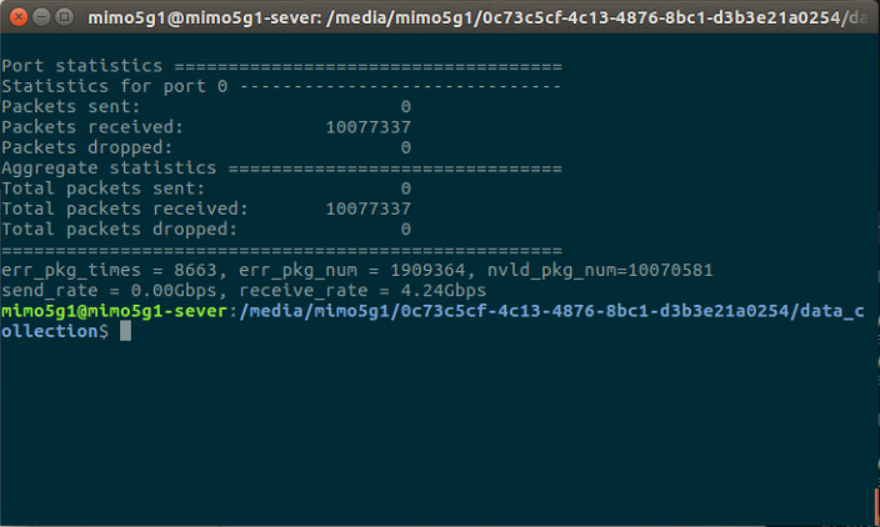
\includegraphics[width = .8\textwidth]{res5ssd.png}
	\caption{向ssd写入}
\end{figure}
\begin{figure}[H]
	\centering
	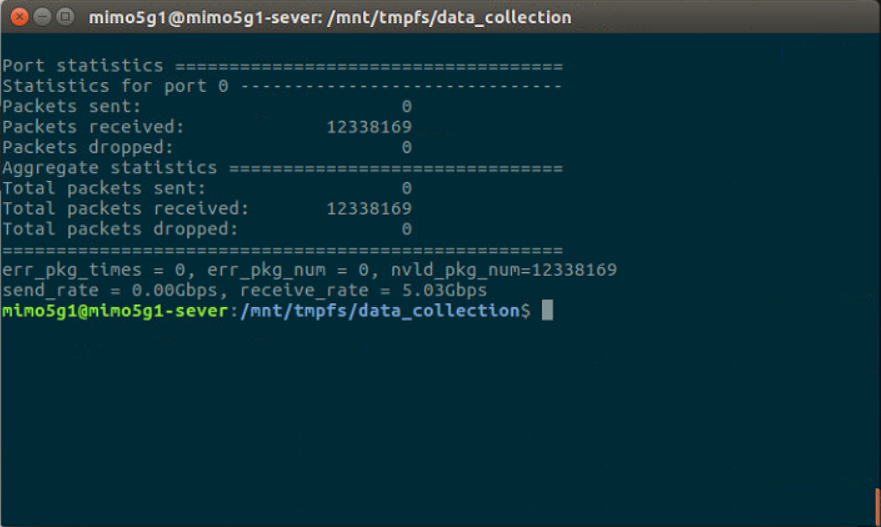
\includegraphics[width = .8\textwidth]{res5ram.png}
	\caption{向tempfs写入}
\end{figure}
\begin{figure}[H]
	\centering
	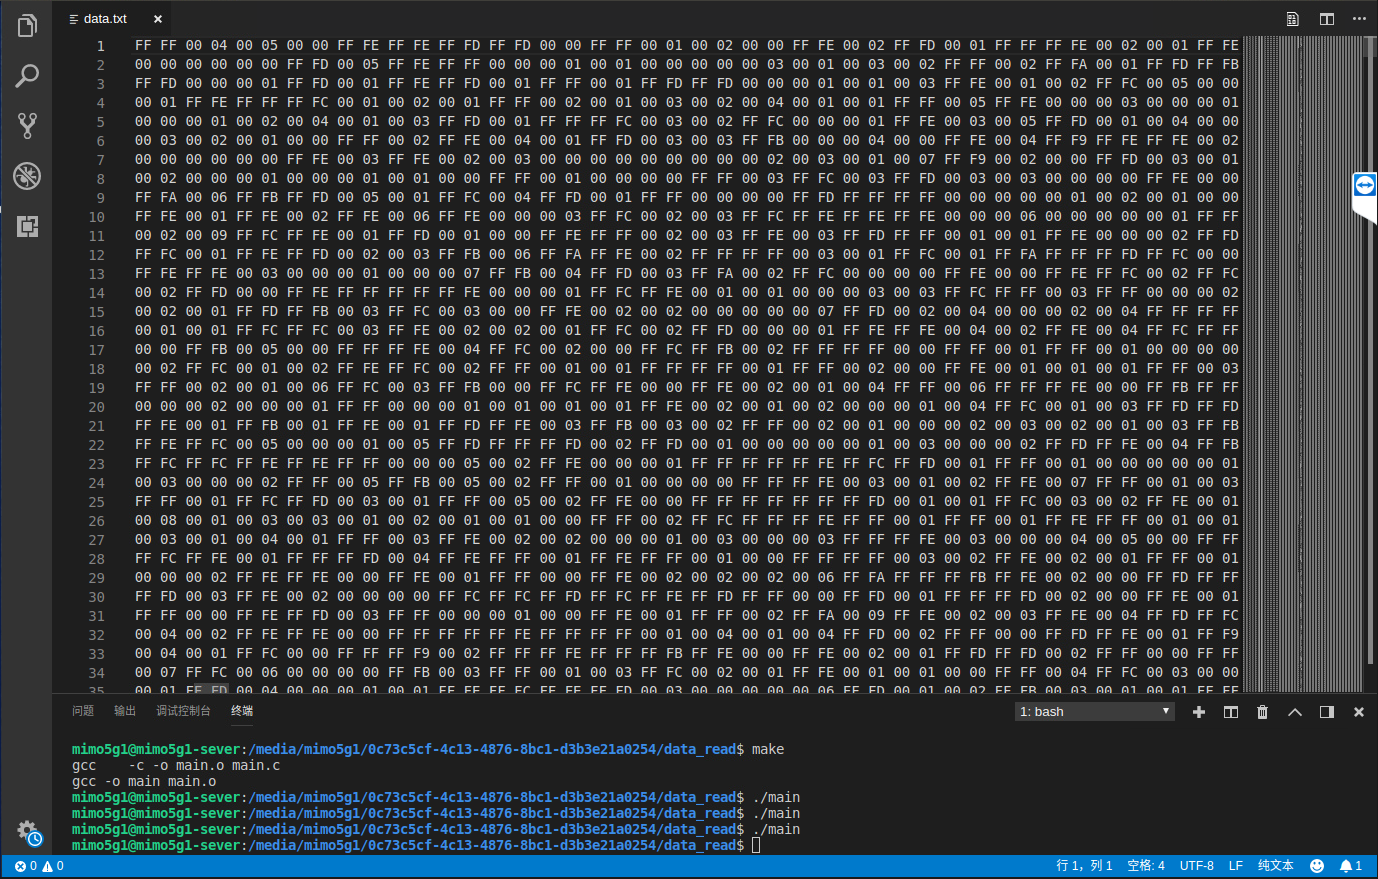
\includegraphics[width = \textwidth]{data.png}
	\caption{转码结果}
\end{figure}

%===========第二节=================
\section{低时延AVX2-LDPC译码实现}
\subsection{设计系统时遇到的问题}
\begin{figure}[H]
	\centering
	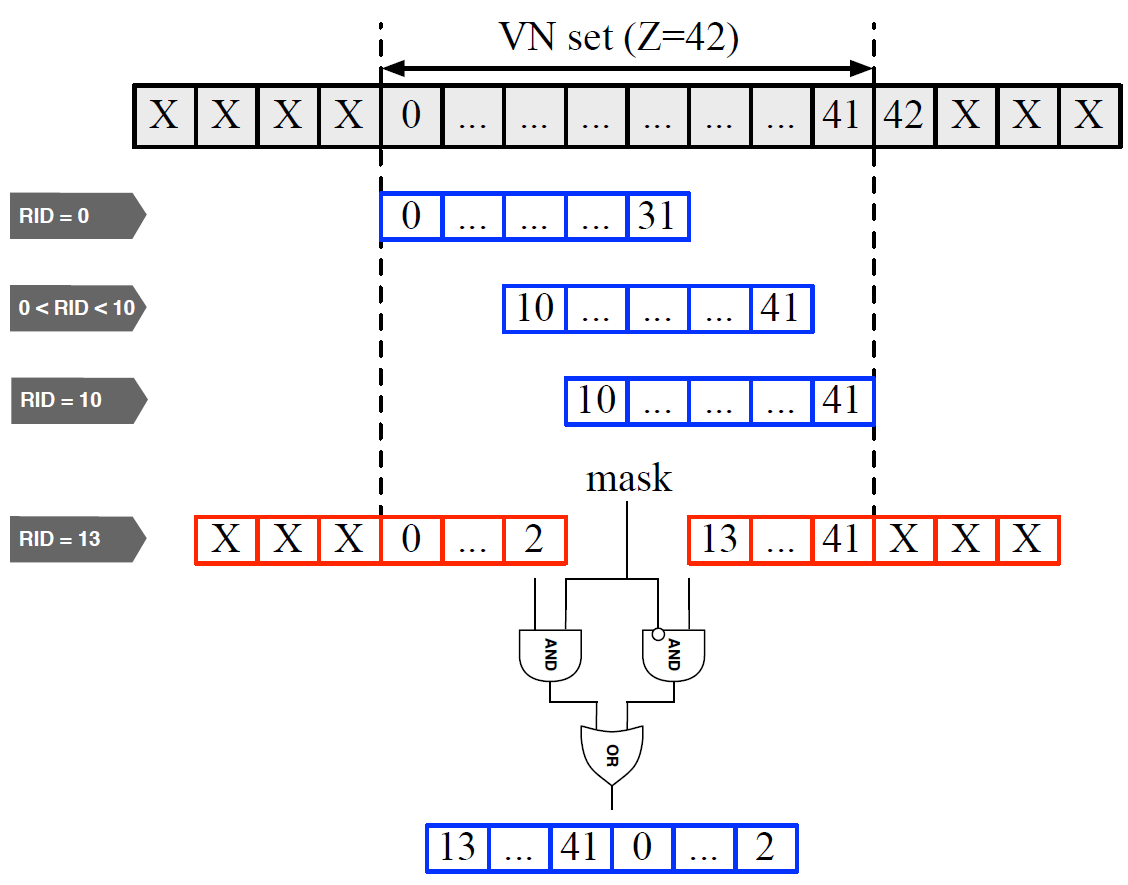
\includegraphics[width = .75\textwidth]{vn.png}
	\caption{论文提到的VN接入方式}
\end{figure}
\begin{figure}[H]
	\centering
	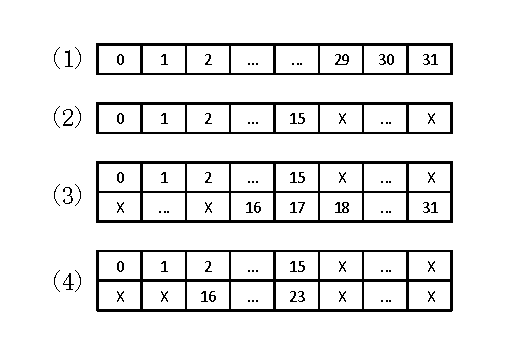
\includegraphics[width = .7\textwidth]{masktype.pdf}
	\caption{实际所有的VN接入方式}
\end{figure}
\subsection{设计的数据结构}
\lstset{language=C++}
\begin{lstlisting}
typedef struct nr15_ldpc_simd_t
{
	…………

	/* Low-Latency Decoder Parameters */
	int32_t units;		// floor(Z_c/REG_SIZE)
	int32_t whole_degree;	// sum of degree of every hbg_row_d
	int8_t* degree;		// number of connective check nodes
				// (length:hbg_row_d)
	__m256i* cn_msg_avx2;	// avx2 message from cn to vn
				// (length:whole_degree*units)
	__m256i* vn_msg_avx2;	// temp avx2 message from vn to cn(length:19)
	int8_t* llr_fixed;	// fixed llr info(length:2*REG_SIZE+Nd)
	int8_t* llr_addr_flag;	// flag for access type
				// (0:no mask;1:1 mask;2:2 mask)
				// (length:whole_degree*units)
	int8_t** llr_addr;	// llr address(length:whole_degree*units)
	int8_t** llr_addr_pre;	// extra llr address for flag=2
				//(length:whole_degree)
	__m256i* mask;		// mask1 for flag=2(length:whole_degree)
	__m256i* mask_pre;	// mask2 for flag=2(length:whole_degree)
	__m256i endmask;	// mask for flag=1

} nr15_ldpc_simd_t;
\end{lstlisting}
\subsection{使用掩码时遇到的问题}
\begin{figure}[H]
	\centering
	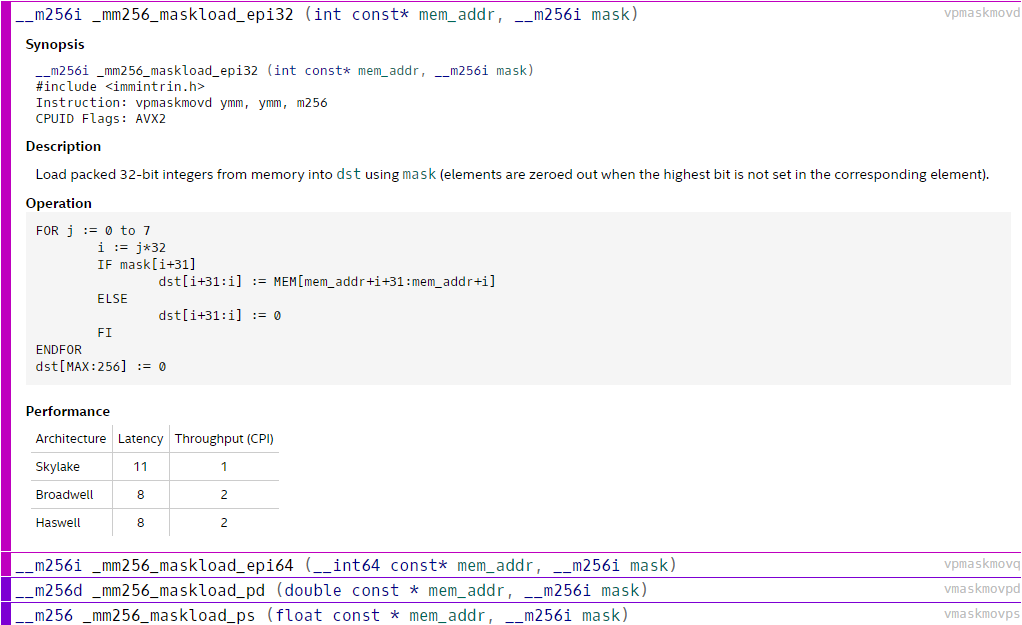
\includegraphics[width = .8\textwidth]{maskload256.png}
	\caption{AVX2 mask load 相关函数}
\end{figure}
\begin{figure}[H]
	\centering
	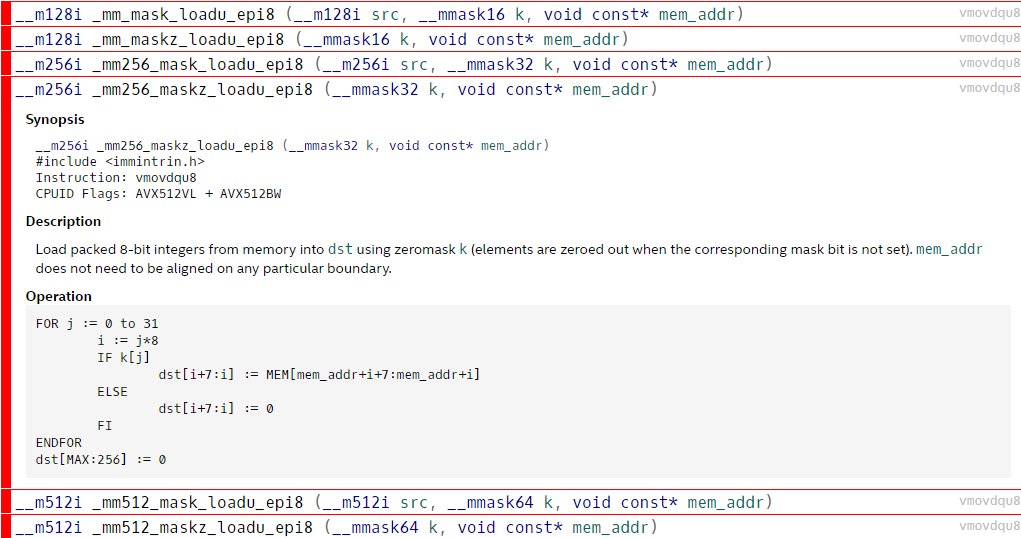
\includegraphics[width = .8\textwidth]{maskload512.png}
	\caption{AVX-512 mask load 相关函数}
\end{figure}
\subsection{当前掩码处理方式}
\subsubsection{取数据加掩码方式}
\begin{lstlisting}
if (*pflag1 == 2)
{
	vllr1 = VECTOR_LOAD(*p_indice_nod1);
	vllr2 = VECTOR_LOAD(*p_indice_nod_pre1);
	mask1 = VECTOR_LOAD(p_mask1);
	mask2 = VECTOR_LOAD(p_maskpre1);
	vllrm1 = VECTOR_AND(vllr1, mask1);
	vllrm2 = VECTOR_AND(vllr2, mask2);
	vllr = VECTOR_OR(vllrm1, vllrm2);

	p_mask1++;
	p_maskpre1++;
	p_indice_nod_pre1++;
}
else
	vllr = VECTOR_LOAD(*p_indice_nod1);
\end{lstlisting}
\subsubsection{存数据加掩码方式}
\begin{lstlisting}
if (*pflag2 == 2)
{
	vllr1 = VECTOR_LOAD(*p_indice_nod2);
	vllr2 = VECTOR_LOAD(*p_indice_nod_pre2);
	mask1 = VECTOR_LOAD(p_mask2);
	mask2 = VECTOR_LOAD(p_maskpre2);
	vllrm1 = VECTOR_AND(mask1, v2llr);
	vllrm2 = VECTOR_AND(mask2, v2llr);
	vllro1 = VECTOR_ANDNOT(mask1, vllr1);
	vllro2 = VECTOR_ANDNOT(mask2, vllr2);
	vllr1 = VECTOR_OR(vllrm1, vllro1);
	vllr2 = VECTOR_OR(vllrm2, vllro2);
	VECTOR_STORE(*p_indice_nod2, vllr1);
	VECTOR_STORE(*p_indice_nod_pre2, vllr2);

	p_mask2++;
	p_maskpre2++;
	p_indice_nod_pre2++;
}
else if (*pflag2 == 1)
{
	vllrm1 = VECTOR_AND(endmask, v2llr);
	vllr = VECTOR_LOAD(*p_indice_nod2);
	vllro1 = VECTOR_ANDNOT(endmask, vllr);						
	vllr = VECTOR_OR(vllrm1, vllro1);
	VECTOR_STORE(*p_indice_nod2, vllr);
}
else
	VECTOR_STORE(*p_indice_nod2, v2llr);
\end{lstlisting}

\subsection{系统测试}
\begin{figure}[H]
	\centering
	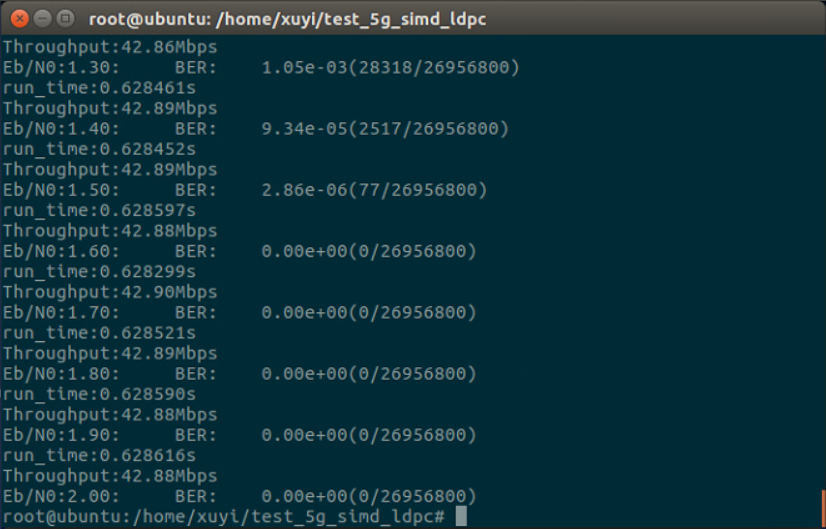
\includegraphics[width = .8\textwidth]{llres.png}
	\caption{运行结果}
\end{figure}
\begin{table}[H]
	\caption{High-Thoughput和Low-Latency系统性能对比(Intel® Xeon® CPU E7-8867 V4 @2.40GHz)}
	\centering
	\begin{tabular}{|l|l|l|l|l|}% 通过添加 | 来表示是否需要绘制竖线
		\hline  % 在表格最上方绘制横线
		scheduling	& High-Thoughput& Low-Latency	\\
		\hline
		Throughput	& 59.19Mbps	& 43.02Mbps	\\
		\hline
		Latency(K=8448)	& 4.5543ms	& 0.1958ms	\\
		\hline  % 在表格最下方绘制横线
	\end{tabular}
\end{table}

%===========第三节=================
\section{改写仿真报告}


%===========第四节=================
% \section{仍存在的问题}


%===========下周计划=================
% \section{下阶段计划}
% 1. 继续完成仿真报告

\end{document}
%%%%%%%%%%%%%%%%%%%%%%%这是正文部分的结束%%%%%%%%%%%%